\jxhj{%教学后记
	}
\skrq{%授课日期
	2017年3月20日 4-5节}
\ktmq{%课题名称
	椭圆弧编程 }
\jxmb{%教学目标,每行前面要加 \item
	\item 掌握siemens上的变量;
	\item 掌握Siemens上的if goto 指令;
	\item 掌握 Siemens上 while endwhile 指令
	\item 会用if then对变量进行修正。 }
\jxzd{%教学重点,每行前面要加 \item
	\item Siemens上变量、if GOTO;
	\item 对变量进行修正。 }
\jxnd{%教学难点,每行前面要加 \item
	\item 对变量进行修正。 }
\jjff{%教学方法
	通过讲述、举例、演示法来说明;}

\makeshouye %制作教案首页

%%%%教学内容
\subsection{组织教学}
\begin{enumerate}[\hspace{2em}1、]
	\item 集中学生注意力;
	\item 清查学生人数;
	\item 维持课堂纪律;
\end{enumerate}
\subsection{复习导入及主要内容}
\begin{enumerate}[\hspace{2em}1、]
\item Z向分层;
\item IF THEN 指令;
\item Z向分层的应用;
\end{enumerate}


\subsection{教学内容及过程}


\subsubsection{相关内容}
\paragraph{变量}
Fanuc: $\#1-\#33 \#100-\#199  \#500-\#999 \#1000$ 以上

Seimens:$ R1-R299 $     开头的系统变量

赋值:Fanuc:$\#101=50$

Seimens: $\#100=50$

引用: Fanuc  $ X\#101   X[\#101*50]$

Siemens$ X=R101  X=R101*50$

\paragraph{运算}

加减乘除

三角函数  $Sin[] Sin() Cos[] cos() tan[] tan()$

单位:度

反三角函数:$ Asin[] Acos[] ATan[]/[]$

$Asin() Acos() Atan2( , )$

$ASin/ACOS $不能大于1
其他函数:

平方根:$SQRT[]  SQRT() $   为正

绝对值:$ABS[]   ABS()$

舍入: $  Round[]  Round() $ 四舍五入

指数:   $EXP[]  exp()   A×10m$

对数:   $LN[]   lN()    logeA$

取整:    上取整  $ Fix[]$ 无条件去小数

Siemens 去小数取整   $Trunc()$

下取整   $Fup[]$  进位取整   
            
\paragraph{条件表达式}
等于:     EQ      =
小于:     LT      <
大于       GT      >
不等于     NE      <>
小于等于   LE      <=
大于等于   GE      >=
\paragraph{流程控制}
A、无条件转移

Fanuc: \verb|GOTO____|

Siemens: GOTO/GOTOB/GOTOF  AA

B、有条件转移

Fanuc: if \[条件表达式\] GOTO

Siemens: IF  条件表达式  GOTO/GOTOB/GOTOF BB

C、循环

Fanuc:  while [条件表达式] DOm

ENDm    m只能为1、2、3

Siemens: while 条件

Endwhile 

\paragraph{值的修正}

Fanuc:  if[条件表达式]then

Siemens: if  条件

Endif

\subsubsection{椭圆弧加工}
参考程序:

零件图如图 \ref{椭圆弧加工} 所示:

	\begin{figure}[!hbtp]
\centering	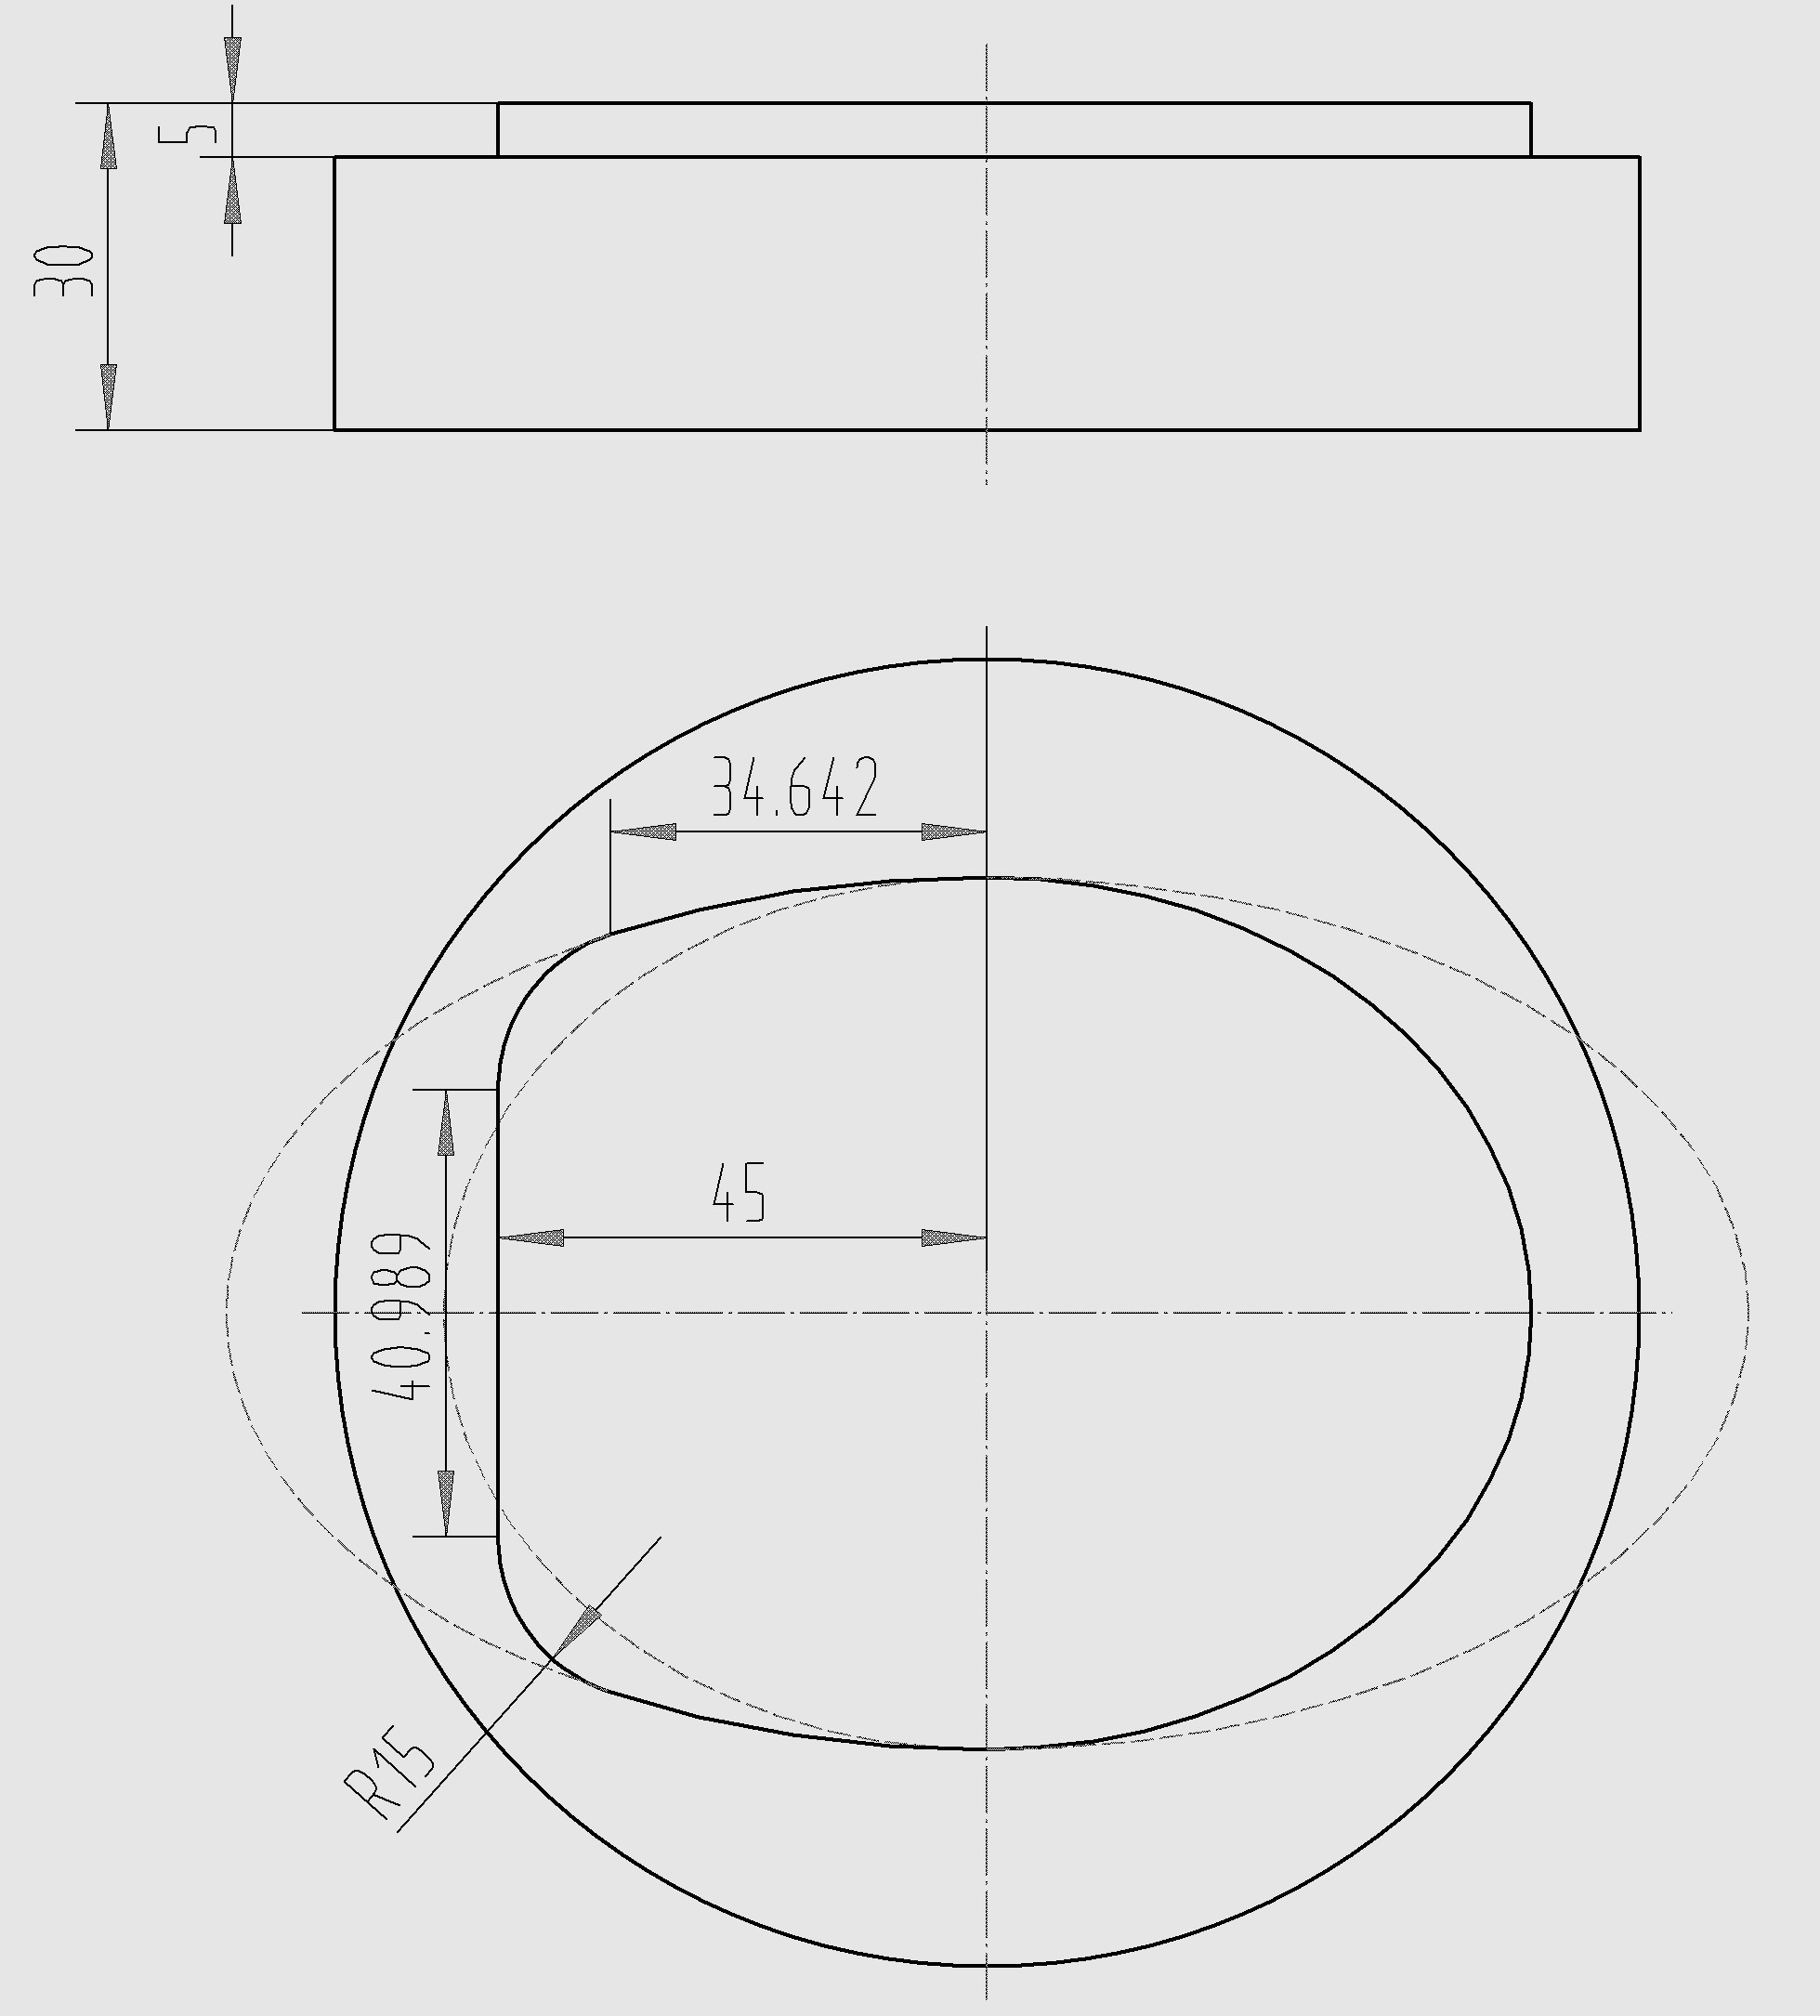
\includegraphics[width=0.8\textwidth]{images/5-1.jpg}
	\caption{椭圆弧加工} \label{椭圆弧加工}
\end{figure}


GX01 \\
G54G17G40G90G64\\
CFC\\
T1D1\\
M3S500\\
G1Z30.F2000\\
X-70.Y0\\
Z5.0\\
Z-5.0F200\\
G1G41X-60.0Y-15.D1\\
G3X-45.Y0R15.\\
G1Y20.495\\
R1=ACOS(-34.642/70)\\
R2=-R1\\
G2 X-34.642  Y=40*SIN(R1)  CR=15.\\
WHILE  R1 >90\\
R1=R1-1\\
G1 X=70*COS(R1)  Y=40*SIN(R1)\\
ENDWHILE\\
WHILE  R1>-90\\
R1=R1-1
G1 X=50*COS(R1)  Y=40*SIN(R1)\\
ENDWHILE\\
WHILE  R1>R2\\
R1=R1-1\\
G1 X=70*COS(R1)  Y=40*SIN(R1)\\
ENDWHILE\\
G2 X-45. Y20.495 R15.\\
G1 Y0\\
G3X-60.Y15.R15.\\
G1G40X-70.Y0\\
Z30.F2000\\
M5\\
M2\\

\subsubsection{应用实例}
正多边形加工思路

	\begin{figure}[!hbtp]
	\centering	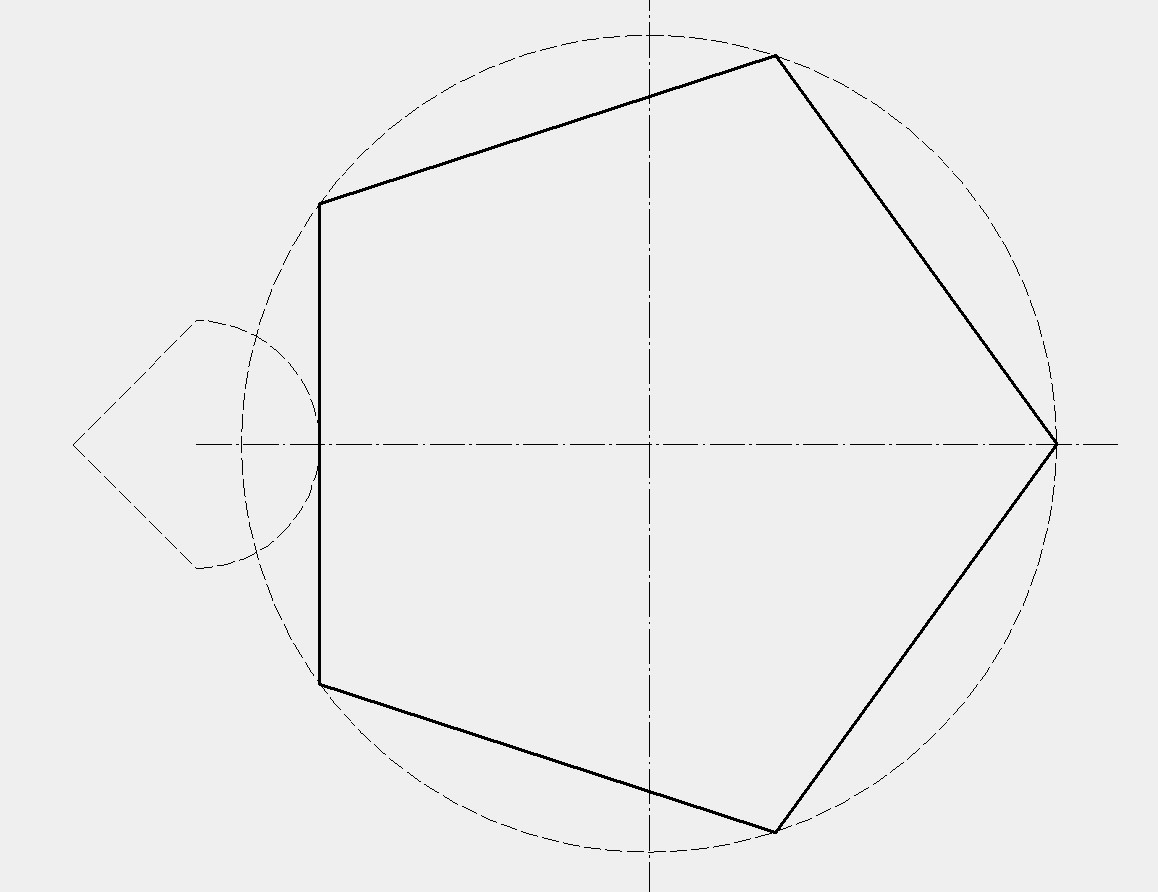
\includegraphics[width=0.8\textwidth]{images/5-2.jpg}
	\caption{正多边形加工} \label{正多边形加工}
\end{figure}

\subsection{课堂小结}
\begin{enumerate}[1、]
	\item 非圆曲线的拟合加工;
	\item 椭圆的数学模型;
	\item 流程控制
	\item 椭圆的宏程序
\end{enumerate}

\vfill
\subsection{布置作业}
\begin{enumerate}[1、]
	\item 编写一个比较通用的外圆加工轮廓。 
\end{enumerate}
\vfill